\documentclass[border=3pt]{standalone}
% Preâmbulo compartilhado pelos diagramas TikZ da aula 5 de IHC (Processos de Design)
\usepackage[T1]{fontenc}
\usepackage[utf8]{inputenc}
\usepackage{lmodern}
\usepackage{amsmath}
\usepackage{xcolor}
\usepackage{tikz}
\usetikzlibrary{arrows.meta,angles,quotes,decorations.pathmorphing,calc,
                positioning,shapes.geometric,shapes.misc,backgrounds,fit,
                math}

% Paleta (mesma dos SVGs originais)
% Paleta da disciplina de IHC: acento roxo (#755099), da capa do livro.
% (o nome "dblue" é mantido para não alterar todos os diagramas)
\definecolor{dblue}{HTML}{755099}
\definecolor{dorange}{HTML}{B3541E}
\definecolor{dgreen}{HTML}{4A7C59}
\definecolor{dred}{HTML}{9C4B4B}
\definecolor{dcream}{HTML}{F4F1EA}
\definecolor{dshade}{HTML}{DDD7C9}

% Função gaussiana (não normalizada por padrão de escala visual)
\pgfmathdeclarefunction{gauss}{3}{%
  \pgfmathparse{1/(#3*sqrt(2*pi))*exp(-((#1-#2)^2)/(2*#3^2))}%
}

% Estilos comuns (prefixo d... para não colidir com chaves internas do pgf)
\tikzset{
  >={Stealth[length=2mm]},
  dguide/.style={gray!55, dashed, line width=0.4pt},
  daxis/.style={gray!60, line width=0.7pt, ->},
  dbody/.style={fill=black!3, draw=black!80, line width=1pt},
  dacc/.style={draw=dblue, line width=1pt},
  dlbl/.style={black!55, font=\small},
  dsub/.style={black!45, font=\footnotesize},
  dstate/.style={circle, draw=black!80, fill=dcream, line width=1pt,
                 minimum size=17mm, font=\large, inner sep=1pt},
  dobs/.style={circle, draw=black!80, fill=dshade, line width=1pt,
               minimum size=14mm, font=\large, inner sep=1pt},
  dbox/.style={rounded corners=2pt, draw=black!80, fill=dcream, line width=1pt,
               align=center, inner sep=6pt},
  dop/.style={circle, draw=black!80, fill=white, line width=1pt,
              minimum size=6mm, inner sep=0pt, font=\small},
  dtrans/.style={->, dblue, line width=1pt},
  dmeas/.style={->, dorange, line width=1pt},
  dcurve/.style={line width=1pt, dblue},
  dcurveb/.style={line width=1.4pt, dorange},
}

\begin{document}
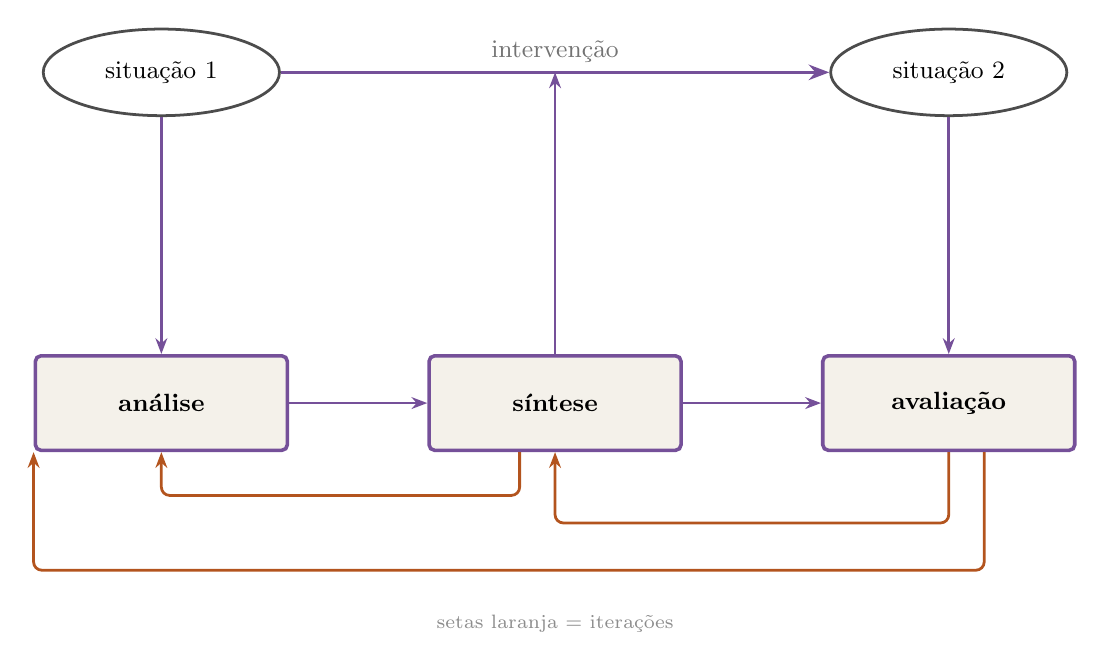
\begin{tikzpicture}[x=1cm,y=1cm,
   act/.style={dbox, minimum width=3.2cm, minimum height=1.2cm, font=\small},
   sit/.style={ellipse, draw=black!70, fill=white, line width=1pt, minimum width=3cm, minimum height=1.1cm, font=\small}]

  \node[sit] (s1) at (0,4.2) {situação 1};
  \node[sit] (s2) at (10,4.2) {situação 2};
  \draw[dtrans, line width=1.3pt, -{Stealth[length=2.6mm]}] (s1.east) -- (s2.west) node[midway, above, dlbl] {intervenção};

  \node[act, draw=dblue, line width=1.3pt] (an) at (0,0) {\textbf{análise}};
  \node[act, draw=dblue, line width=1.3pt] (si) at (5,0) {\textbf{síntese}};
  \node[act, draw=dblue, line width=1.3pt] (av) at (10,0) {\textbf{avaliação}};

  \draw[dtrans] (s1) -- (an);
  \draw[dtrans] (si.north) -- (5,4.2);
  \draw[dtrans] (s2) -- (av);
  \draw[dtrans] (an) -- (si);
  \draw[dtrans] (si) -- (av);

  \draw[dmeas, rounded corners=3pt] (av.south) -- ++(0,-0.9) -| (si.south);
  \draw[dmeas, rounded corners=3pt] (si.south) ++(-0.45,0) -- ++(0,-0.55) -| (an.south);
  \draw[dmeas, rounded corners=3pt] (av.south) ++(0.45,0) -- ++(0,-1.5) -| (an.south west);

  \node[dsub, font=\scriptsize, align=center, text width=7cm] at (5,-2.8) {setas laranja = iterações};

\end{tikzpicture}
\end{document}
